% Graphic for TeX using PGF
% Title: /media/danilo/E472BA7972BA5052/Danilo/Documenti/Università/LatexTesiMagistrale/images/meshes.dia
% Creator: Dia v0.97.3
% CreationDate: Fri Jan 29 10:28:45 2016
% For: danilo
% \usepackage{tikz}
% The following commands are not supported in PSTricks at present
% We define them conditionally, so when they are implemented,
% this pgf file will use them.
\ifx\du\undefined
  \newlength{\du}
\fi
\setlength{\du}{15\unitlength}
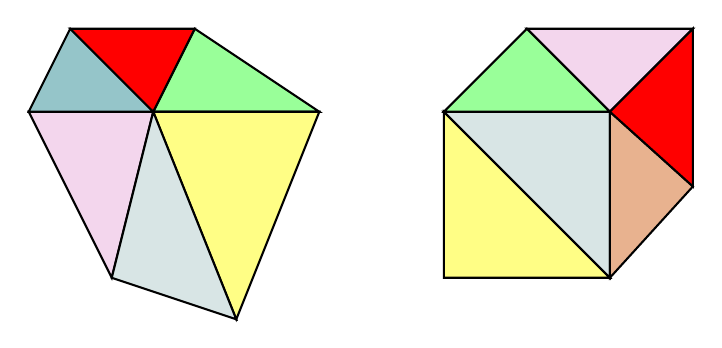
\begin{tikzpicture}
\pgftransformxscale{1.000000}
\pgftransformyscale{-1.000000}
\definecolor{dialinecolor}{rgb}{0.000000, 0.000000, 0.000000}
\pgfsetstrokecolor{dialinecolor}
\definecolor{dialinecolor}{rgb}{1.000000, 1.000000, 1.000000}
\pgfsetfillcolor{dialinecolor}
\pgfsetlinewidth{0.050000\du}
\pgfsetdash{}{0pt}
\pgfsetdash{}{0pt}
\pgfsetmiterjoin
\pgfsetbuttcap
\definecolor{dialinecolor}{rgb}{0.952941, 0.839216, 0.929412}
\pgfsetfillcolor{dialinecolor}
\fill (18.000000\du,5.000000\du)--(21.000000\du,5.000000\du)--(20.000000\du,9.000000\du)--cycle;
\definecolor{dialinecolor}{rgb}{0.000000, 0.000000, 0.000000}
\pgfsetstrokecolor{dialinecolor}
\draw (18.000000\du,5.000000\du)--(21.000000\du,5.000000\du)--(20.000000\du,9.000000\du)--cycle;
\pgfsetlinewidth{0.050000\du}
\pgfsetdash{}{0pt}
\pgfsetdash{}{0pt}
\pgfsetmiterjoin
\pgfsetbuttcap
\definecolor{dialinecolor}{rgb}{0.600000, 1.000000, 0.600000}
\pgfsetfillcolor{dialinecolor}
\fill (21.000000\du,5.000000\du)--(25.000000\du,5.000000\du)--(22.000000\du,3.000000\du)--cycle;
\definecolor{dialinecolor}{rgb}{0.000000, 0.000000, 0.000000}
\pgfsetstrokecolor{dialinecolor}
\draw (21.000000\du,5.000000\du)--(25.000000\du,5.000000\du)--(22.000000\du,3.000000\du)--cycle;
\pgfsetlinewidth{0.050000\du}
\pgfsetdash{}{0pt}
\pgfsetdash{}{0pt}
\pgfsetmiterjoin
\pgfsetbuttcap
\definecolor{dialinecolor}{rgb}{0.584314, 0.772549, 0.788235}
\pgfsetfillcolor{dialinecolor}
\fill (18.000000\du,5.000000\du)--(21.000000\du,5.000000\du)--(19.000000\du,3.000000\du)--cycle;
\definecolor{dialinecolor}{rgb}{0.000000, 0.000000, 0.000000}
\pgfsetstrokecolor{dialinecolor}
\draw (18.000000\du,5.000000\du)--(21.000000\du,5.000000\du)--(19.000000\du,3.000000\du)--cycle;
\pgfsetlinewidth{0.050000\du}
\pgfsetdash{}{0pt}
\pgfsetdash{}{0pt}
\pgfsetmiterjoin
\pgfsetbuttcap
\definecolor{dialinecolor}{rgb}{1.000000, 0.000000, 0.000000}
\pgfsetfillcolor{dialinecolor}
\fill (19.000000\du,3.000000\du)--(22.000000\du,3.000000\du)--(21.000000\du,5.000000\du)--cycle;
\definecolor{dialinecolor}{rgb}{0.000000, 0.000000, 0.000000}
\pgfsetstrokecolor{dialinecolor}
\draw (19.000000\du,3.000000\du)--(22.000000\du,3.000000\du)--(21.000000\du,5.000000\du)--cycle;
\pgfsetlinewidth{0.050000\du}
\pgfsetdash{}{0pt}
\pgfsetdash{}{0pt}
\pgfsetmiterjoin
\pgfsetbuttcap
\definecolor{dialinecolor}{rgb}{1.000000, 0.996078, 0.521569}
\pgfsetfillcolor{dialinecolor}
\fill (21.000000\du,5.000000\du)--(25.000000\du,5.000000\du)--(23.000000\du,10.000000\du)--cycle;
\definecolor{dialinecolor}{rgb}{0.000000, 0.000000, 0.000000}
\pgfsetstrokecolor{dialinecolor}
\draw (21.000000\du,5.000000\du)--(25.000000\du,5.000000\du)--(23.000000\du,10.000000\du)--cycle;
\pgfsetlinewidth{0.050000\du}
\pgfsetdash{}{0pt}
\pgfsetdash{}{0pt}
\pgfsetmiterjoin
\pgfsetbuttcap
\definecolor{dialinecolor}{rgb}{0.847059, 0.898039, 0.898039}
\pgfsetfillcolor{dialinecolor}
\fill (20.000000\du,9.000000\du)--(21.000000\du,5.000000\du)--(23.000000\du,10.000000\du)--cycle;
\definecolor{dialinecolor}{rgb}{0.000000, 0.000000, 0.000000}
\pgfsetstrokecolor{dialinecolor}
\draw (20.000000\du,9.000000\du)--(21.000000\du,5.000000\du)--(23.000000\du,10.000000\du)--cycle;
\pgfsetlinewidth{0.050000\du}
\pgfsetdash{}{0pt}
\pgfsetdash{}{0pt}
\pgfsetmiterjoin
\pgfsetbuttcap
\definecolor{dialinecolor}{rgb}{1.000000, 0.996078, 0.521569}
\pgfsetfillcolor{dialinecolor}
\fill (28.000000\du,5.000000\du)--(32.000000\du,9.000000\du)--(28.000000\du,9.000000\du)--cycle;
\definecolor{dialinecolor}{rgb}{0.000000, 0.000000, 0.000000}
\pgfsetstrokecolor{dialinecolor}
\draw (28.000000\du,5.000000\du)--(32.000000\du,9.000000\du)--(28.000000\du,9.000000\du)--cycle;
\pgfsetlinewidth{0.050000\du}
\pgfsetdash{}{0pt}
\pgfsetdash{}{0pt}
\pgfsetmiterjoin
\pgfsetbuttcap
\definecolor{dialinecolor}{rgb}{0.847059, 0.898039, 0.898039}
\pgfsetfillcolor{dialinecolor}
\fill (28.000000\du,5.000000\du)--(32.000000\du,9.000000\du)--(32.000000\du,5.000000\du)--cycle;
\definecolor{dialinecolor}{rgb}{0.000000, 0.000000, 0.000000}
\pgfsetstrokecolor{dialinecolor}
\draw (28.000000\du,5.000000\du)--(32.000000\du,9.000000\du)--(32.000000\du,5.000000\du)--cycle;
\pgfsetlinewidth{0.050000\du}
\pgfsetdash{}{0pt}
\pgfsetdash{}{0pt}
\pgfsetmiterjoin
\pgfsetbuttcap
\definecolor{dialinecolor}{rgb}{0.952941, 0.839216, 0.929412}
\pgfsetfillcolor{dialinecolor}
\fill (30.000000\du,3.000000\du)--(32.000000\du,5.000000\du)--(34.000000\du,3.000000\du)--cycle;
\definecolor{dialinecolor}{rgb}{0.000000, 0.000000, 0.000000}
\pgfsetstrokecolor{dialinecolor}
\draw (30.000000\du,3.000000\du)--(32.000000\du,5.000000\du)--(34.000000\du,3.000000\du)--cycle;
\pgfsetlinewidth{0.050000\du}
\pgfsetdash{}{0pt}
\pgfsetdash{}{0pt}
\pgfsetmiterjoin
\pgfsetbuttcap
\definecolor{dialinecolor}{rgb}{0.600000, 1.000000, 0.600000}
\pgfsetfillcolor{dialinecolor}
\fill (30.000000\du,3.000000\du)--(28.000000\du,5.000000\du)--(32.000000\du,5.000000\du)--cycle;
\definecolor{dialinecolor}{rgb}{0.000000, 0.000000, 0.000000}
\pgfsetstrokecolor{dialinecolor}
\draw (30.000000\du,3.000000\du)--(28.000000\du,5.000000\du)--(32.000000\du,5.000000\du)--cycle;
\pgfsetlinewidth{0.050000\du}
\pgfsetdash{}{0pt}
\pgfsetdash{}{0pt}
\pgfsetmiterjoin
\pgfsetbuttcap
\definecolor{dialinecolor}{rgb}{0.909804, 0.698039, 0.560784}
\pgfsetfillcolor{dialinecolor}
\fill (32.000000\du,9.000000\du)--(34.000000\du,6.800000\du)--(32.000000\du,5.000000\du)--cycle;
\definecolor{dialinecolor}{rgb}{0.000000, 0.000000, 0.000000}
\pgfsetstrokecolor{dialinecolor}
\draw (32.000000\du,9.000000\du)--(34.000000\du,6.800000\du)--(32.000000\du,5.000000\du)--cycle;
\pgfsetlinewidth{0.050000\du}
\pgfsetdash{}{0pt}
\pgfsetdash{}{0pt}
\pgfsetmiterjoin
\pgfsetbuttcap
\definecolor{dialinecolor}{rgb}{1.000000, 0.000000, 0.000000}
\pgfsetfillcolor{dialinecolor}
\fill (34.000000\du,3.000000\du)--(34.000000\du,6.800000\du)--(32.000000\du,5.000000\du)--cycle;
\definecolor{dialinecolor}{rgb}{0.000000, 0.000000, 0.000000}
\pgfsetstrokecolor{dialinecolor}
\draw (34.000000\du,3.000000\du)--(34.000000\du,6.800000\du)--(32.000000\du,5.000000\du)--cycle;
\end{tikzpicture}
